\documentclass[10pt,a4paper]{article}
\usepackage[utf8]{inputenc}
\usepackage[T1]{fontenc}
\IfFileExists{brazil.ldf}{\usepackage[brazil]{babel}}{\renewcommand{\refname}{Referências}}
\usepackage[margin=2cm]{geometry}
\usepackage{booktabs,tabularx,array,graphicx}
\usepackage[hidelinks]{hyperref}
\usepackage[expansion=false]{microtype}
\setlength{\parindent}{0pt}
\setlength{\parskip}{5pt}
\newcolumntype{Y}{>{\raggedright\arraybackslash}X}
\title{Warm-start da otimização de Random Forest\\em regressão desbalanceada}
\author{Carlos Henrique Dias\\\small IN1097 --- Atividade prática 3}
\date{}

\begin{document}
\maketitle
\vspace{-0.5cm}
\begin{center}\small
Código público, notebook com saídas e matriz de perdas:\\
\url{https://github.com/carloshendvpm/projeto01-mtl/tree/entrega-pratica-03/pratica-03}
\end{center}

\section{Problema e objetivo}

Em regressão desbalanceada, alguns valores do alvo são pouco representados, embora sejam importantes para o problema. Por isso, avaliamos as previsões com a Squared Error--Relevance Area (SERA), que dá maior importância aos erros em valores relevantes, sem deixar de considerar o restante do domínio \cite{ribeiro}. Nas práticas anteriores, usamos características dos datasets para recomendar regressores. Nesta atividade, mantemos o problema e os datasets, mas fixamos um regressor e investigamos por onde começar a busca de seus hiperparâmetros.

O trabalho se apoia no Meta-IR, de Avelino, Cavalcanti e Cruz \cite{metair}, que recomenda regressor e estratégia de reamostragem a partir de meta-características. Os autores utilizam regressores com hiperparâmetros padrão e apontam a otimização como uma possível extensão. O estudo anterior dos mesmos autores \cite{resampling} também fundamenta a avaliação por SERA no domínio. Aqui, adotamos a inicialização por datasets similares de Feurer et al.\ \cite{feurer}: configurações boas em problemas parecidos são usadas como primeiros pontos de uma busca baseada em modelo.

A pergunta é: \textbf{as meta-características estendidas da Prática 2 ajudam a encontrar mais rapidamente boas configurações de Random Forest?} Para responder, é necessário distinguir duas explicações: a similaridade entre datasets pode orientar a escolha, ou podem simplesmente existir configurações geralmente boas. Por isso, comparamos o warm-start por similaridade com uma inicialização por rank médio, que não consulta as características do alvo. Esta atividade adapta essas ideias a um regressor fixo; não reproduz integralmente o Meta-IR.

\section{Dados e espaço de configurações}

Reutilizamos os 30 datasets de regressão desbalanceada das práticas anteriores. Escolhemos Random Forest como regressor base por ser um dos modelos do Meta-IR e ter obtido o melhor rank médio por SERA na nossa matriz anterior sem reamostragem, aproximadamente 1,73 entre seis regressores. Essa escolha não garante que ele seja o mais sensível à otimização. O treinamento utiliza os dados originais, sem acrescentar busca sobre reamostragem.

Investigamos somente dois hiperparâmetros, relacionados à construção das árvores \cite{probst}. A grade é fixa, transparente e igual em todos os datasets:

\begin{center}\small
\begin{tabularx}{\linewidth}{lYY}
\toprule
Hiperparâmetro & O que controla & Valores \\
\midrule
\texttt{max\_features} & Proporção de atributos candidatos por divisão & 1,0; 0,2; 0,35; 0,5; 0,65; 0,8 \\
\texttt{min\_samples\_leaf} & Mínimo de exemplos em uma folha & 1; 2; 3; 4; 5; 6; 8; 10; 12; 16 \\
\bottomrule
\end{tabularx}
\end{center}

São $K=60$ combinações, incluindo o padrão da biblioteca: proporção de atributos igual a 1,0 e mínimo de um exemplo por folha. Mantemos 100 árvores, semente 42 e os demais hiperparâmetros no padrão. A grade cobre desde o uso de todos os atributos até uma fração de 0,2 e de folhas unitárias a folhas de 16 exemplos, variando a aleatoriedade e a regularização. O espaçamento mais denso em folhas pequenas explora alterações próximas ao padrão, mantendo o custo de 60 configurações. Essas faixas são escolhas do experimento.

O protocolo usa dez folds, com embaralhamento e semente 42, iguais para todas as configurações. A perda de cada configuração é a SERA média dos folds. Mantemos a convenção da implementação anterior: relevância automática, considerando ambas as caudas, calculada no alvo do fold avaliado para pontuar as previsões. Ela não participa do treinamento do Random Forest. A SERA é o objetivo externo da busca; o regressor continua sendo ajustado pelo seu critério padrão de erro quadrático.

A matriz completa tem 60 linhas, uma por configuração, e 30 colunas, uma por dataset. Sua construção exigiu $60\times30\times10=18.000$ ajustes. As buscas foram simuladas por consultas à tabela, sem novos treinos. A passagem final da construção, retomada de checkpoints, levou 85,5 minutos de parede com seis processos; a soma dos tempos registrados nos ajustes foi 8,40 horas. Esse tempo de parede não inclui a tentativa interrompida anterior. A SERA foi calculada pela mesma soma trapezoidal com passo 0,01, reutilizando os pesos de relevância por fold; a equivalência com a função legada foi verificada nos dez folds do piloto.

\section{Warm-start e protocolo de comparação}

Cada busca teve orçamento de $T=20$ avaliações, incluindo $n_{\mathrm{init}}=5$ pontos iniciais, e foi repetida com vinte sementes. Assim, $K=3T$, atendendo ao tamanho mínimo pedido no enunciado. As sementes repetem a busca sobre uma mesma tabela de perdas, e não o treinamento dos regressores.

Para cada dataset alvo, adotamos leave-one-dataset-out: somente os outros 29 datasets podem fornecer rankings, configurações iniciais e parâmetros de pré-processamento das meta-características. Comparamos cinco estratégias:

\begin{center}\small
\begin{tabularx}{\linewidth}{lY}
\toprule
Estratégia & Funcionamento \\
\midrule
Configuração padrão & Referência fixa, sem busca. \\
Random search & Sorteia vinte configurações distintas. \\
SMBO frio & Começa com cinco configurações aleatórias e continua com o modelo substituto. \\
SMBO por similaridade & Começa com configurações bem avaliadas nos datasets mais próximos do alvo. \\
SMBO por rank médio & Começa com as cinco configurações de melhor rank médio nos datasets de treino. \\
\bottomrule
\end{tabularx}
\end{center}

Nos três SMBO, mantemos o mesmo processo gaussiano e a mesma função de aquisição, expected improvement. O modelo usa apenas as perdas já observadas no alvo. Cada sugestão deve ser uma configuração ainda não avaliada e consome uma avaliação. Para tornar o protocolo reproduzível, fixamos o kernel Matérn com $\nu=2{,}5$ e escala 0,5, sem otimização desses parâmetros, com \texttt{alpha=1e-6} e normalização das perdas observadas. A configuração é representada pela proporção de atributos e pelo logaritmo de base 2 do tamanho mínimo de folha, dividido por 4.

Comparamos duas representações do dataset. \textbf{Xbase} contém os 13 descritores anteriores. \textbf{Xestendido} acrescenta 38 medidas de complexidade dos grupos global, normal e raro, totalizando 51 descritores. Reutilizamos as 36 medidas locais de complexidade e reconstruímos T2 dos normais e dos raros pela razão exemplos/atributos multiplicada pela proporção do grupo, preservando as 51 colunas da representação dos três grupos da Prática 2. T2 do conjunto completo já está na base; as colunas de diagnóstico ficam de fora. Usamos os valores locais disponíveis, não as saídas históricas do Colab: a extração prévia subamostrou 13 datasets em cinco réplicas de 1.500 exemplos; as 36 colunas têm 16 valores ausentes, tratados no protocolo abaixo.

A similaridade é medida pela distância euclidiana após padronização. A mediana para preencher valores indefinidos e a escala são ajustadas somente nos datasets de treino; colunas inteiramente indefinidas nesse treino são descartadas. Variamos o número de vizinhos em $k=1,3,5$. Percorremos a melhor configuração de cada vizinho, depois a segunda melhor e assim por diante, até obter cinco configurações distintas. O braço principal, definido antes dos resultados, é Xestendido com $k=3$.

\section{Resultados}

\subsection{Eficiência da busca}
A perda em cada passo é a melhor SERA já observada, normalizada entre o mínimo e o máximo da tabela para cada dataset. A AUC é a média dos vinte pontos dessa curva; menor é melhor. Primeiro agregamos as vinte sementes por dataset e depois os trinta datasets, dando o mesmo peso a cada problema. O padrão é uma referência fixa ao longo do orçamento.

\begin{center}\small
\begin{tabular}{lrrrr}
\toprule
Método & AUC & Aval. 5 & Aval. 12 & Aval. 20 \\
\midrule
Padrão & 0,1652 & 0,1652 & 0,1652 & 0,1652 \\
Random search & 0,1000 & 0,1309 & 0,0665 & 0,0356 \\
SMBO frio & 0,0705 & 0,1309 & 0,0211 & 0,0111 \\
Rank médio & 0,0288 & 0,0292 & 0,0183 & 0,0146 \\
Similaridade (estendido, k=3) & 0,0206 & 0,0255 & 0,0179 & 0,0095 \\
\bottomrule
\end{tabular}
\end{center}

\begin{center}
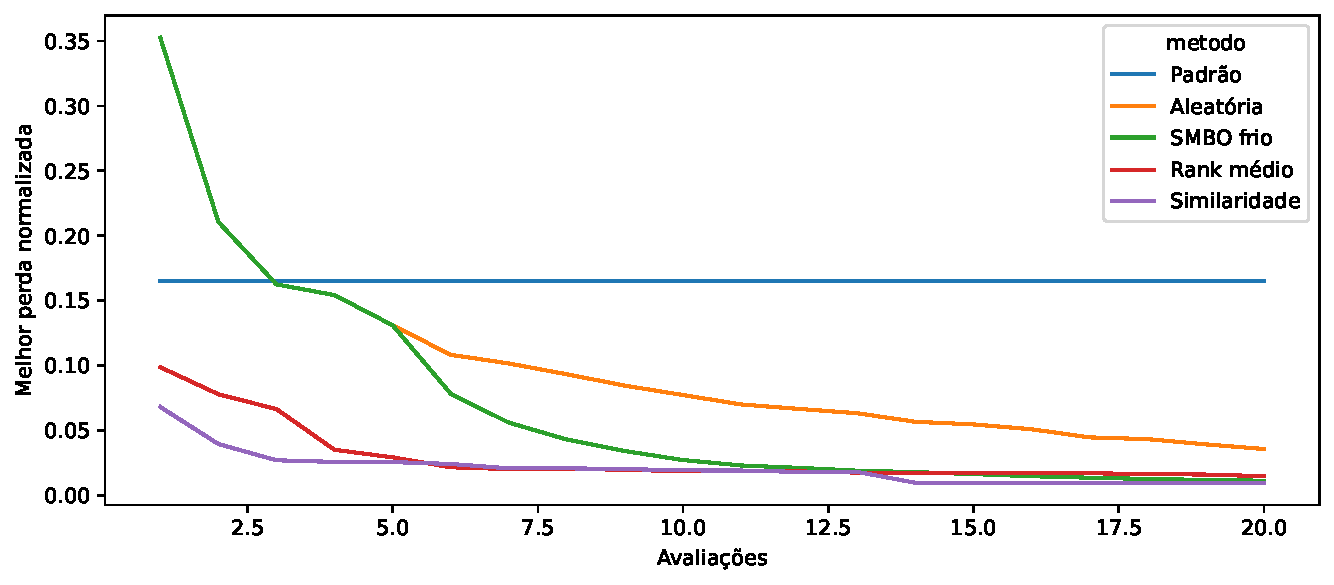
\includegraphics[width=.60\linewidth]{resultados/curvas.pdf}
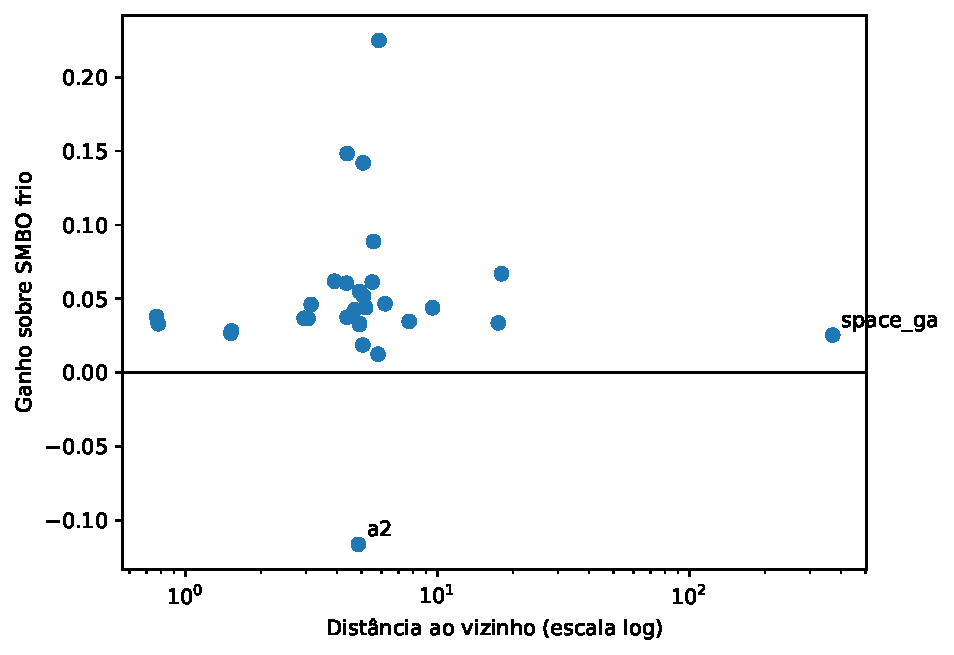
\includegraphics[width=.36\linewidth]{resultados/distancia_ganho.pdf}
\end{center}

A similaridade principal reduziu a AUC em 70,8\% frente ao SMBO frio (0,0705 para 0,0206; Nemenyi, $p=0,0014$). Após cinco avaliações, as perdas médias eram 0,0255 e 0,1309, respectivamente, com diferença significativa ($p=1,52\times10^{-8}$). Nos passos 12 e 20, as diferenças entre esses métodos deixaram de ser significativas ($p=0,582$ e $p=0,994$), apesar da menor média final da similaridade. Portanto, o benefício estatisticamente sustentado está na inicialização e na eficiência acumulada; não há evidência de vantagem final sobre o SMBO frio. O modelo substituto permitiu ao frio recuperar boa parte da diferença inicial.

Aplicamos Friedman sobre os trinta datasets, agregando as sementes antes de cada teste. Os valores de $p$ foram AUC: $p=2,78\times 10^{-14}$; 5: $p=1,76\times 10^{-15}$; 12: $p=1,30\times 10^{-16}$; 20: $p=1,65\times 10^{-18}$. Os diagramas apresentam os ranks médios e os grupos sem diferença significativa pelo pós-teste de Nemenyi ($\alpha=0,05$); ausência de significância não demonstra equivalência.

\begin{center}
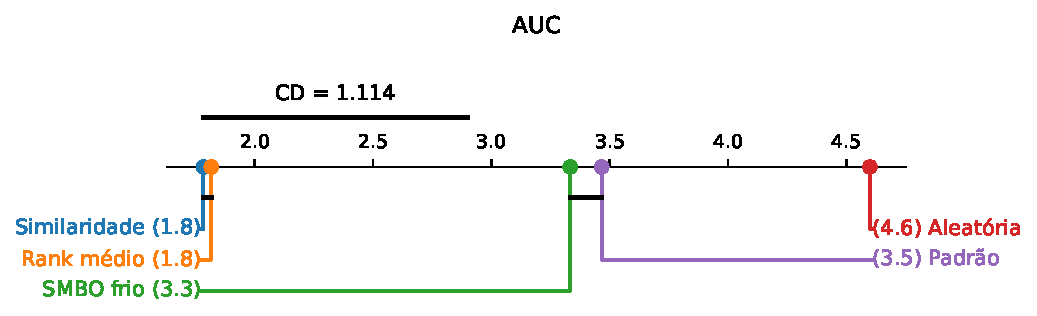
\includegraphics[width=.82\linewidth]{resultados/cd_auc.pdf}\par
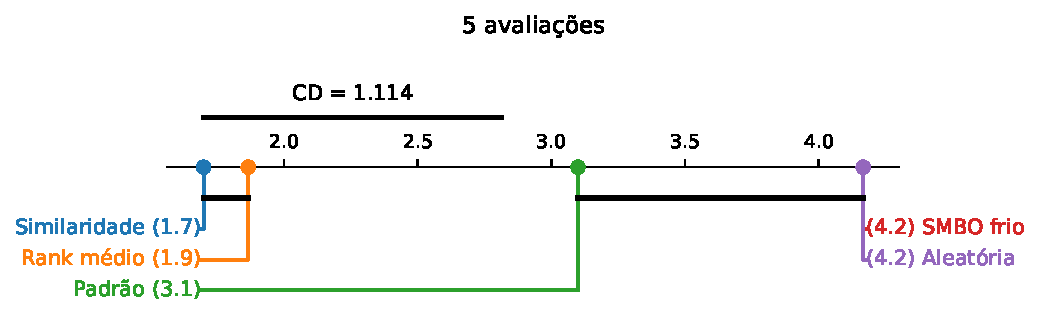
\includegraphics[width=.82\linewidth]{resultados/cd_5.pdf}\par
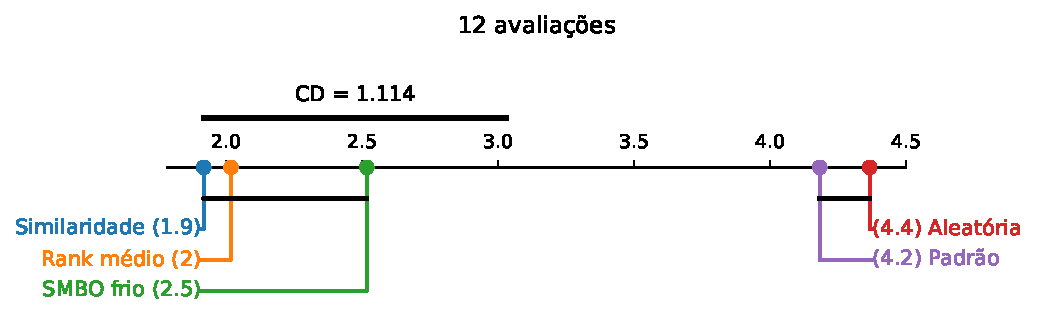
\includegraphics[width=.82\linewidth]{resultados/cd_12.pdf}\par
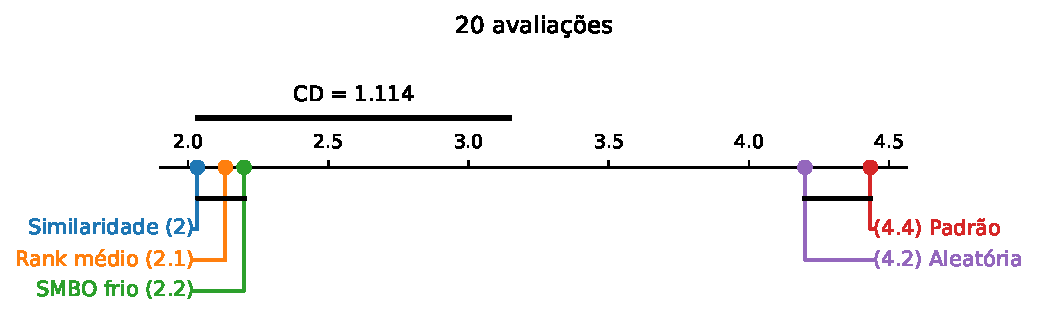
\includegraphics[width=.82\linewidth]{resultados/cd_20.pdf}\par
\end{center}

\subsection{O papel das meta-características}
A tabela apresenta todas as representações e valores de $k$. Ganhos positivos indicam menor AUC que o respectivo controle. O braço principal continua sendo Xestendido com $k=3$, definido antes de examinar os resultados.

\begin{center}\small
\begin{tabular}{lrrrr}
\toprule
Representação & $k$ & AUC & Ganho sobre frio & Ganho sobre rank \\
\midrule
Base & 1 & 0,0236 & 0,0469 & 0,0052 \\
Base & 3 & 0,0226 & 0,0479 & 0,0062 \\
Base & 5 & 0,0165 & 0,0540 & 0,0123 \\
Estendido & 1 & 0,0188 & 0,0516 & 0,0099 \\
Estendido & 3 & 0,0206 & 0,0499 & 0,0082 \\
Estendido & 5 & 0,0217 & 0,0488 & 0,0070 \\
\bottomrule
\end{tabular}
\end{center}

O rank médio também supera o frio na AUC ($p=0,0019$). Similaridade e rank médio não se distinguem significativamente na AUC nem nos três orçamentos (todos os $p>0,99$). Logo, não conseguimos atribuir a vantagem sobre a partida fria às meta-características: um portfólio de configurações geralmente boas continua sendo uma explicação compatível com os dados. Isso não demonstra equivalência entre as inicializações.

A extensão melhora a média em $k=1$ e $k=3$, mas piora em $k=5$. A menor AUC descritiva é de Xbase/$k=5$ (0,0165), enquanto Xestendido/$k=5$ obtém 0,0217. Não há melhora consistente ao acrescentar os descritores; as comparações das seis variantes são descritivas, sem declarar significância nem substituir o braço principal após observar os resultados. A extensão também acrescenta colunas correlacionadas e razões já deriváveis da base, alterando a ponderação da distância.

\subsection{Quando o warm-start falha}
Definimos o ganho por dataset como AUC do frio menos AUC da similaridade principal. O warm-start apresentou ganho positivo em 29 datasets, negativo em 1 e empate numérico em 0. A correlação de Spearman entre ganho e distância ao vizinho mais próximo foi $\rho=0,150$ ($p=0,428$). A associação é um diagnóstico, sem interpretação causal. A tabela mostra os três menores ganhos, com os vizinhos e pontos iniciais efetivamente utilizados.

\begin{center}\scriptsize
\begin{tabularx}{\linewidth}{lYYr}
\toprule
Dataset & Três vizinhos & Cinco configurações iniciais & Ganho \\
\midrule
a2 & a7, kdd\_coil\_1, boston & c030, c050, c010, c031, c000 & -0,1164 \\
analcatdata\_apnea3 & forestFires, meta, abalone & c011, c012, c000, c023, c022 & 0,0125 \\
meta & forestFires, analcatdata\_apnea3, heat & c011, c040, c023, c050, c021 & 0,0187 \\
\bottomrule
\end{tabularx}
\end{center}

Apenas \texttt{a2} teve transferência negativa. Seus vizinhos \texttt{a7}, \texttt{kdd\_coil\_1} e \texttt{boston} têm ótimos com folha de tamanho 1; as cinco iniciais transferidas usam folhas 1 ou 2. Já o ótimo de \texttt{a2}, c033, combina proporção de atributos 0,5 e folha 4. A melhor inicial ocupa somente o 12º rank no alvo. O SMBO explora outras folhas, mas não avalia c033 no orçamento disponível: termina com perda normalizada 0,2861, contra 0,0969 do frio. Sua AUC é 0,2927, contra 0,1763 do frio. A proximidade nas meta-características não assegurou a transferência das preferências de configuração, e a continuação não corrigiu essa desvantagem em vinte passos.

Os outros dois casos da tabela ainda têm ganho positivo; são contrastes de baixo benefício, não falhas. A distância de \texttt{a2} (4,85) não é extrema, enquanto \texttt{space\_ga}, com distância 370,29, ainda tem ganho positivo de 0,0254. A correlação e a dispersão, com distâncias em escala logarítmica, não sustentam usar apenas essa distância para prever falhas.

\section{Interpretação e limites}
O warm-start acelerou o início da busca e melhorou a AUC em 29 dos 30 datasets; os maiores ganhos foram em \texttt{a3} (0,2251), \texttt{kdd\_coil\_1} (0,1484) e \texttt{a7} (0,1421). A vantagem sobre a partida fria não persistiu estatisticamente até o orçamento final. O controle por rank médio impede atribuir o ganho exclusivamente à similaridade, e a extensão das meta-características não trouxe melhora consistente entre os valores de $k$.

Para a pesquisa em seleção dinâmica de modelos para regressão desbalanceada, levaria o controle por portfólio e a verificação de que descritores por grupo predizem diferenças de desempenho, além de descreverem os problemas. Este resultado em HPO de um regressor fixo não estabelece seu efeito sobre competência local. Antes de ampliar a representação, investigaria sua redundância e a estabilidade das vizinhanças em validação entre datasets.

O ótimo é restrito às 60 configurações: uma região promissora fora da grade não pode ser descoberta. O orçamento cobre um terço da tabela e as curvas medem eficiência nesse espaço discreto. As perdas após seleção não estimam de forma independente a generalização do modelo escolhido, o que exigiria avaliação externa ou validação aninhada. As sementes variam a busca sobre a mesma tabela, não os treinos da matriz. Os tempos da matriz não incluem a extração anterior das meta-características nem permitem concluir sobre aceleração total em segundos. Xestendido acrescenta complexidade global, normal e rara, portanto seu efeito não isola a contribuição dos valores raros. Os testes principais comparam cinco métodos; a análise das seis variantes de representação e $k$ é descritiva.

\begin{thebibliography}{9}
\small
\bibitem{metair} Avelino, J. G.; Cavalcanti, G. D. C.; Cruz, R. M. O. Imbalanced Regression Pipeline Recommendation. 2025. \url{https://arxiv.org/abs/2507.11901}.
\bibitem{resampling} Avelino, J. G.; Cavalcanti, G. D. C.; Cruz, R. M. O. Resampling strategies for imbalanced regression: a survey and empirical analysis. \textit{Artificial Intelligence Review}, 57, 82, 2024. \url{https://doi.org/10.1007/s10462-024-10724-3}.
\bibitem{feurer} Feurer, M.; Springenberg, J. T.; Hutter, F. Initializing Bayesian Hyperparameter Optimization via Meta-Learning. \textit{AAAI}, 2015. \url{https://doi.org/10.1609/aaai.v29i1.9354}.
\bibitem{probst} Probst, P.; Wright, M. N.; Boulesteix, A.-L. Hyperparameters and tuning strategies for random forest. \textit{WIREs Data Mining and Knowledge Discovery}, 9, e1301, 2019. \url{https://doi.org/10.1002/widm.1301}.
\bibitem{ribeiro} Ribeiro, R. P.; Moniz, N. Imbalanced regression and extreme value prediction. \textit{Machine Learning}, 109, 1803--1835, 2020. \url{https://doi.org/10.1007/s10994-020-05900-9}.
\end{thebibliography}
\end{document}
